\section{RV12 Execution Pipeline}

The RV12 implements a 32/64bit Integer RISC pipeline. The pipeline consists of the Instruction Fetch, Pre-Decode, Instruction Decode, Execution, and Write Back stages.
 

\begin{figure}[h]
  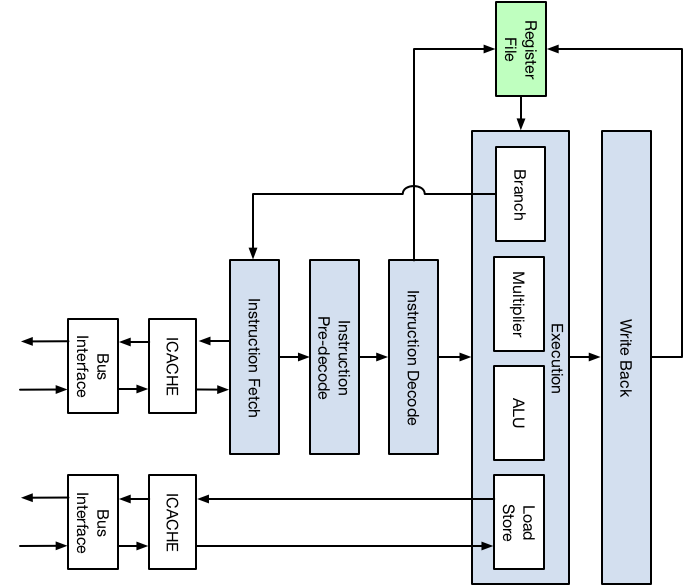
\includegraphics{Pipeline-Overview}
  \caption{RV12 Execution Pipeline}
\end{figure}

\pagebreak

\subsection{Instruction Fetch (IF)}\label{instruction-fetch-if}

\begin{figure}[h]
  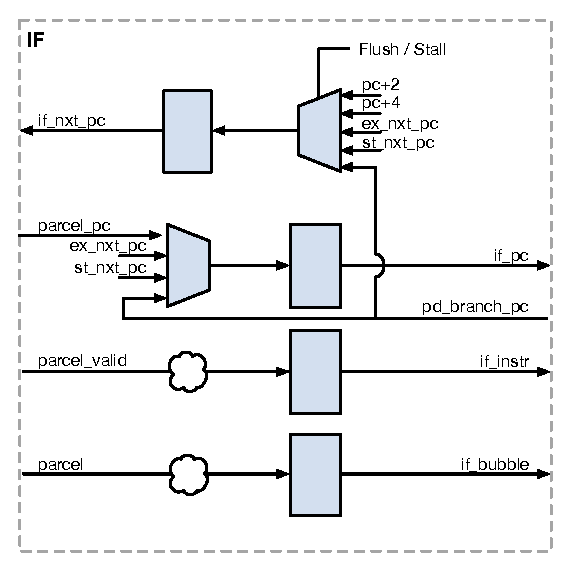
\includegraphics{Pipeline-IF.eps}
  \caption{Instruction Fetch Stage Implementation}
\end{figure}

The Instruction Fetch unit loads a new parcel from the program memory.
A parcel is a code field that contains one or more instructions. The address of the parcel to load is held by the Program Counter (PC). The Program Counter is either 32 or 64bits wide, depending on the XLEN parameter. The Program Counter is updated whenever the Instruction Pipeline is not stalled.

In case the pipeline must be flushed the Program Counter is restarted from the given address.

\pagebreak

\subsection{Pre-Decode (PD)}\label{pre-decode-pd}

The Pre-Decode unti translates 16-bit compressed instructions to the base 32bit RISC-V instructions and then processes Program Counter modifying instructions. Jump-And-Link and Branch instructions modify the Program Counter in the Instruction Fetch stage. This avoids waiting for the Execution stage to trigger the update and reduces the demand for pipeline flushes.
The destination address for branches is predicted based on the data provided by the optional Branch Prediction Unit or determined statically based on the offset.


\begin{figure}[th]
  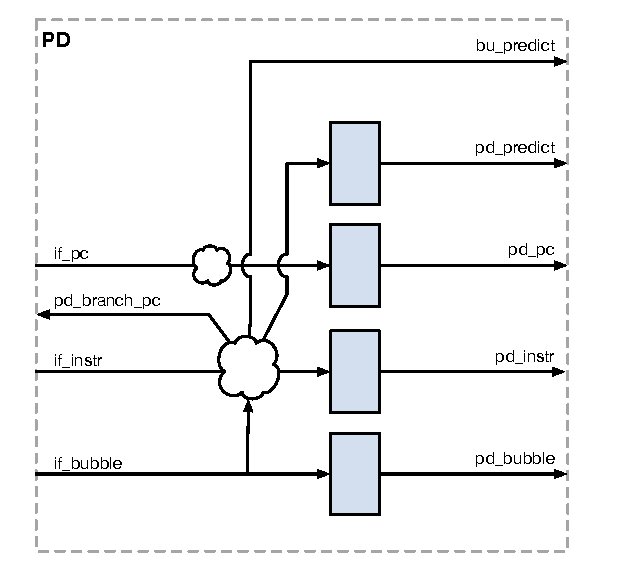
\includegraphics{Pipeline-PD.eps}
  \caption{Instruction Pre-Decode Stage}
\end{figure}

\pagebreak

\subsection{Instruction Decode (ID)}\label{instruction-decode-id-1}

The Instruction Decode unit ensures the operands for the execution units
are available. It accesses the Register File, calculates immediate
values, and sets bypasses.

\begin{figure}[h]
  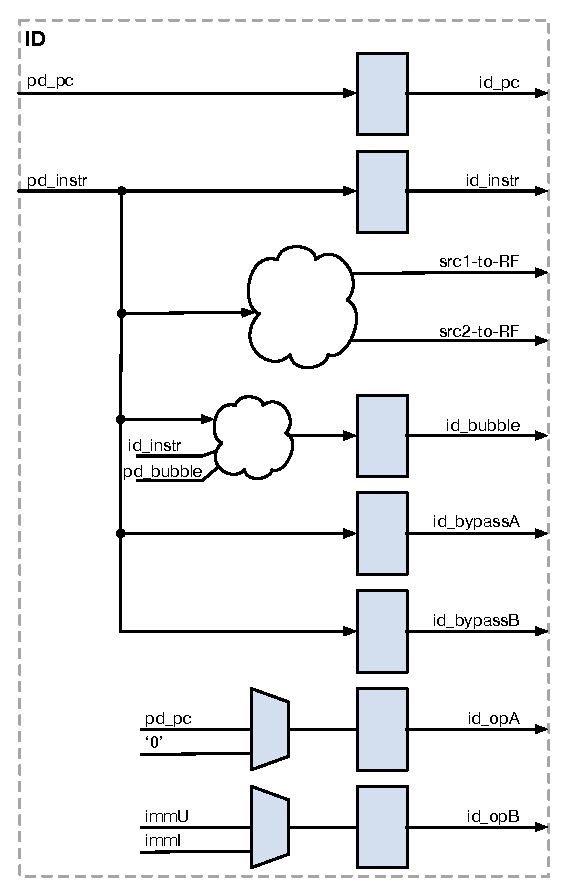
\includegraphics{Pipeline-ID.eps}
  \caption{Instruction Decode Stage Implementation}
\end{figure}

\pagebreak

\subsection{Execute (EX)}\label{execute-ex-1}

The Execute stage performs the required operation on the data provided by the Instruction Decode stage. The Execution stage has multiple execution units, each with a unique function;
The ALU performs logical and arithmetic operations.
The Multiplier unit calculates signed/unsigned multiplications.
The Divider unit calculates signed/unsigned division and remainder.
The Load-Store Unit accesses the data memory.
The Branch Unit calculates jump and branch addresses and validates the predicted branches.

Only one operation can be executed per clock cycle.
Most operations complete in one clock cycle, except for the divide instructions, which always take multiple clock cycles to complete. The multiplier supports configurable latencies, to improve performance.


\begin{figure}[h]
  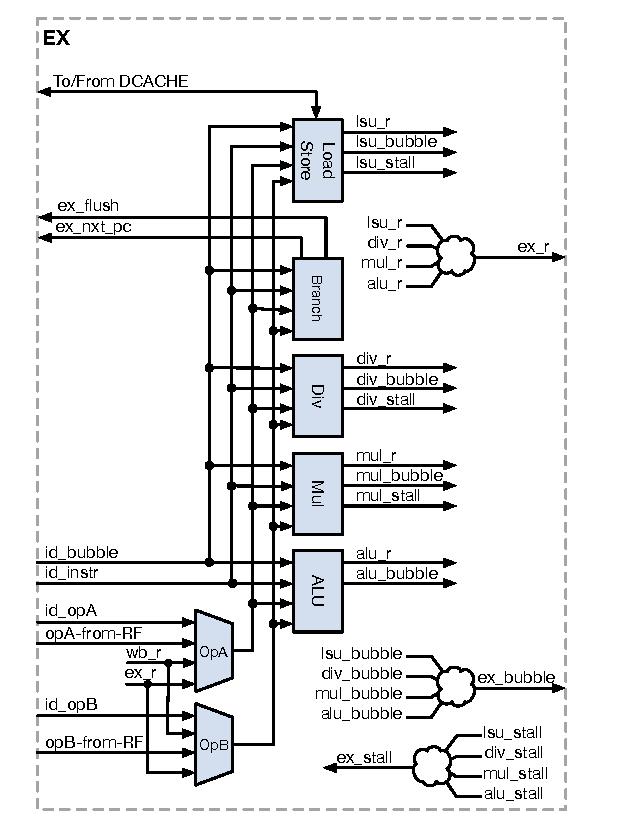
\includegraphics{Pipeline-EX.eps}
  \caption{Execute Stage Implementation}
\end{figure}

\pagebreak

\subsection{Write-Back (WB)}\label{write-back-wb-1}

The Write-Back stage writes the results from the Execution Unit into the Register File.

\begin{figure}[h]
  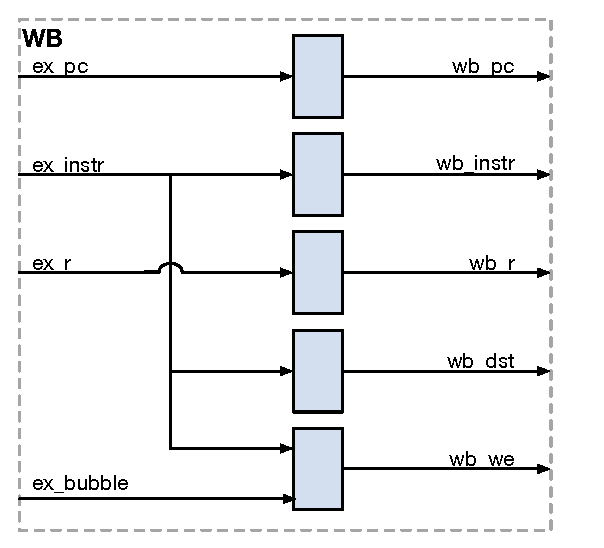
\includegraphics{Pipeline-WB.eps}
  \caption{Write-back Stage Implementation}
\end{figure}
